\subsection{Perbaikan Algoritma CART}

Kesalahan yang dilakukan pada implementasi sebelumnya yaitu pada penggunaan
atribut untuk pemisahan \textit{tree}.
Jika sebuah atribut telah digunakan sebagai pemisah, dan menjadi sebuah
\textit{node} pada pohon keputusan, maka atribut tersebut tidak boleh diproses
atau menjadi pemisah kembali pada anak-anaknya, namun bisa diproses kembali
pada \textit{grandchild}-nya.

Hal seperti ini tidak pernah disebutkan dalam teks algoritma CART,
sehingga saya cukup kesulitan menemukan kesalahan yang dilakukan.

Hasil implementasi dibandingkan dengan package CART dari program \texttt{R}
dengan menggunakan dataset Iris.

Berikut \textit{tree} dari hasil implementasi sendiri,

\begin{lstlisting}
CART Tree:
 { petal-length false true 150 2 2.45}
        { petal-width false true 100 3 1.75}
                { petal-length false true 46 2 4.85}
                        {Iris-virginica  true false 43 0 <nil>}
                        { sepal-length false true 3 0 5.95}
                                {Iris-virginica  true false 2 0 <nil>}
                                {Iris-versicolor  true false 1 0 <nil>}
                { petal-length false true 54 2 4.95}
                        { petal-width false true 6 3 1.55}
                                { sepal-length false true 3 0 6.95}
                                        {Iris-virginica  true false 1 0 <nil>}
                                        {Iris-versicolor  true false 2 0 <nil>}
                                {Iris-virginica  true false 3 0 <nil>}
                        { petal-width false true 48 3 1.65}
                                {Iris-virginica  true false 1 0 <nil>}
                                {Iris-versicolor  true false 47 0 <nil>}
        {Iris-setosa  true false 50 0 <nil>}
\end{lstlisting}

Berikut \textit{tree} menggunakan package \texttt{rpart} dari program \texttt{R},

\begin{lstlisting}
 1) root 150 100 setosa (0.33333333 0.33333333 0.33333333)
   2) Petal.Length< 2.45 50   0 setosa (1.00000000 0.00000000 0.00000000) *
   3) Petal.Length>=2.45 100  50 versicolor (0.00000000 0.50000000 0.50000000)
     6) Petal.Width< 1.75 54   5 versicolor (0.00000000 0.90740741 0.09259259)
      12) Petal.Length< 4.95 48   1 versicolor (0.00000000 0.97916667 0.02083333)
        24) Petal.Width< 1.65 47   0 versicolor (0.00000000 1.00000000 0.00000000) *
        25) Petal.Width>=1.65 1   0 virginica (0.00000000 0.00000000 1.00000000) *
      13) Petal.Length>=4.95 6   2 virginica (0.00000000 0.33333333 0.66666667)
        26) Petal.Width>=1.55 3   1 versicolor (0.00000000 0.66666667 0.33333333)
          52) Sepal.Length< 6.95 2   0 versicolor (0.00000000 1.00000000 0.00000000) *
          53) Sepal.Length>=6.95 1   0 virginica (0.00000000 0.00000000 1.00000000) *
        27) Petal.Width< 1.55 3   0 virginica (0.00000000 0.00000000 1.00000000) *
     7) Petal.Width>=1.75 46   1 virginica (0.00000000 0.02173913 0.97826087)
      14) Petal.Length< 4.85 3   1 virginica (0.00000000 0.33333333 0.66666667)
        28) Sepal.Length< 5.95 1   0 versicolor (0.00000000 1.00000000 0.00000000) *
        29) Sepal.Length>=5.95 2   0 virginica (0.00000000 0.00000000 1.00000000) *
      15) Petal.Length>=4.85 43   0 virginica (0.00000000 0.00000000 1.00000000) *
\end{lstlisting}

Hasil dari kedua \textit{tree} sama.

\subsection{Implementasi Random Forest}

Implemetansi algoritma \textit{ensemble} \textit{Random Forest} (RF) secara
umum mengacu pada buku Friedman, dkk. \cite{friedman2001elements}, dengan
tambahan dari video kuliah dan tulisan lain di internet.

Algoritma RF yang diimplementasikan menggunakan teknik \textit{bagging},
\textit{out-of-bag} (OOB), dan CART sebagai pengklasifikasi di setiap pohon
keputusan.

\clearpage

Berikut algoritma RF yang digunakan,

\begin{lstlisting}
FUNGSI RandomForest
INPUT
	D: dataset
	NTREE: jumlah tree
	NFEATURE: jumlah fitur yang dipilih secara acak
	NBAGGING: jumlah sub-sampel yang dipilih secara acak dengan
	replacement, dalam nilai persentase.
OUTPUT
	FOREST: kumpulan tree
VAR
	SUMOOBERROR: total galat untuk OOB
BEGIN
	SUMOOBERROR := 0.0

	FOR i = 0; i < NTREE; i++
	BEGIN
		bootstrap, oob := RandomPickRows(D, NBAGGING)

		cartTree := CreateTree(bootstrap, NFEATURE)

		ooberror := cartTree.CountOOBError(oob)

		SUMOOBERROR += ooberror

		FOREST.AddTree(cartTree)
	END

	FOREST.AverageOOBError = SUMOOBERROR / NTREE
END
\end{lstlisting}

Hasil implementasi kemudian diuji dengan dataset,
\begin{itemize}
\item \textit{Glass Identification}
\cite{evett1987rule}, dengan jumlah sampel yaitu 124, jumlah fitur 9, jumlah
kelas yaitu 7 (contoh data bisa dilihat pada lampiran
\ref{appendix:dataset_glass}).
Hasilnya dalam bentuk grafik penghitungan laju galat OOB yang dapat dilihat
pada gambar \ref{fig:rf_glass}.

\item \textit{Iris}, dengan jumlah sampel yaitu 150, jumlah fitur 5, jumlah
kelas 3.
Hasilnya dalam bentuk grafik penghitungan laju galat OOB yang dapat dilihat
pada gambar \ref{fig:rf_iris}.
\end{itemize}

\begin{figure}[t]
	\centering
	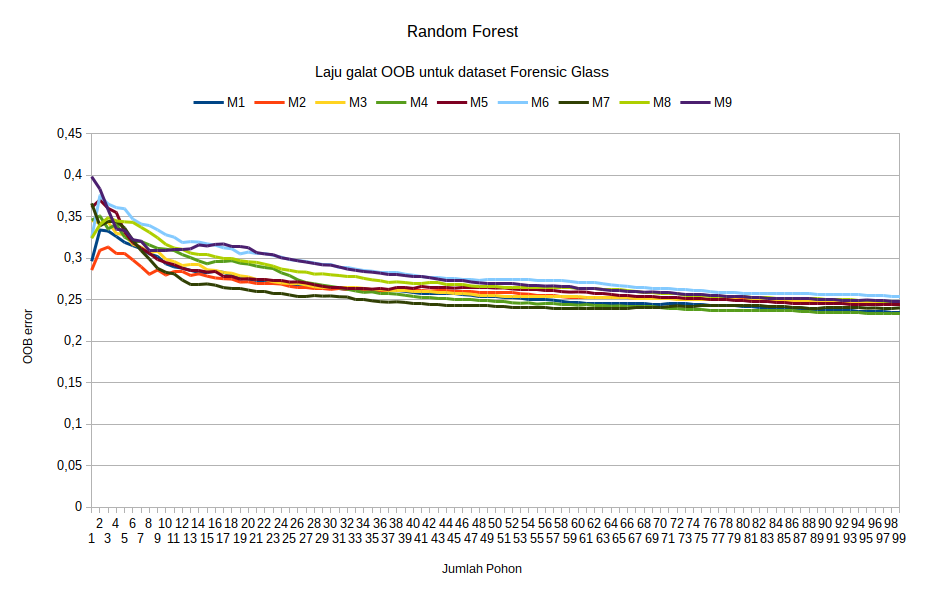
\includegraphics[keepaspectratio=true,scale=0.5]{rf_glass}
	\caption{Laju galat OOB pada \textit{Random Forest} untuk dataset
	\textit{Forensic Glass} dengan jumlah fitur acak dari 2 sampai 9.
	M1-M9 yaitu jumlah fitur acak yang digunakan, yang mana M2 berarti dua
	fitur acak dipilih, M3 berarti tiga fitur acak dipilih, dst.
	}
	\label{fig:rf_glass}
\end{figure}

\begin{figure}[t]
	\centering
	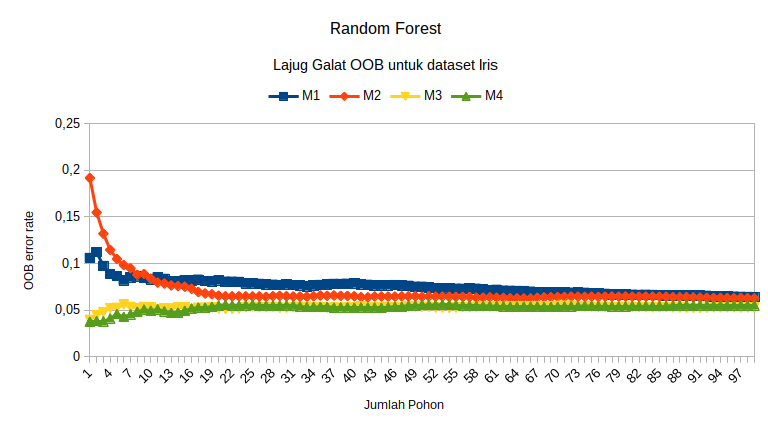
\includegraphics[keepaspectratio=true,scale=0.5]{rf_iris}
	\caption{Laju galat OOB pada \textit{Random Forest} untuk dataset
	\textit{Iris} dengan jumlah fitur acak dari 1 sampai 4.}
	\label{fig:rf_iris}
\end{figure}


Dataset diuji dengan mengambil dua per tiga (66\%) dari data asli untuk
\textit{bootstrap} dan sisanya digunakan sebagai latihan (OOB) untuk
mendapatkan galat, dengan jumlah tree yang digunakan yaitu 50.
